% This will be the main document for the Technical Networks paper to
% be written by the Eggnet team of Jordan Ell, Triet Huynh and Braden
% Simpson in association with Adrian Schroeter and Daniela Damian.

\documentclass[conference]{IEEEtran}

% Use of outside images
\usepackage{graphicx} 

% Correct bad hyphenation here
\hyphenation{op-tical net-works semi-conduc-tor}

% Begin the paper here
\begin{document}


% Paper title
% Can use linebreaks \\ within to get better formatting as desired
\title{Software Failure Prediction With Changeset Technical Dependencies}

% Author names
% Use a multiple column layout for up to three different affiliations
\author{\IEEEauthorblockN{Jordan Ell}
\IEEEauthorblockA{University of Victoria\\
Victoria, British Columbia\\
jell@uvic.ca}
\and
\IEEEauthorblockN{Triet Huynh}
\IEEEauthorblockA{University of Victoria\\
Vancouver, British Columbia\\
infiro@uvic.ca}
\and
\IEEEauthorblockN{Braden Simpson}
\IEEEauthorblockA{University of Victoria\\
Victoria, British Columbia\\
braden@uvic.ca}}

% Make the title area
\maketitle


\begin{abstract}
Software systems have not only become larger over time, but the amount of
technical contributors and dependencies have also increased. With these expansions also comes
the increasing risk of introducing a software failure into a pre-existing system.
Software failures are a multi-billion dollar problem in the industry today and while integration and
other forms of testing are helping to ensure a minimal number of failures, research to understand
full impacts of changesets and their social implications is still a major concern. This paper describes
how analysis of changesets and the technical relationships they infer can be used to detect when failures 
may occur and between what contributors the failures are induced. The result of these predictions
also provide a communication recommendation per changeset that supports the notion of
socio-technical congruence which is know to increase changeset success.
\end{abstract}


\section{Introduction}

% Setup the problem.
Often, large software projects are created using highly modular and 
reusable code. The problem this creates, is that methods or functions\footnote{This includes object constructors} 
can be used in a wide variety of locations throughout the project creating many technical 
dependencies.  This causes changes to any given method inside the project to have a rippling 
effect across the rest of the project\cite{Acharya:2011:PCI}. The larger these effects are,
the more likely they are to cause a software failure inside the system during the project's
life span\cite{Zimmermann:2008:PDU}. These observations open the door to many types
of network analysis in regard to technical dependencies and preventing software failures.

% Explain technical network research that already exists
Research has shown, that technical dependencies inside of a project can be used as a major
tool for predicting the success or failure of changesets or builds \cite{Pinzger:2008:DNP}
\cite{Zimmermann:2008:PDU}. However, most research in this area is based off of identifying
central modules inside of a large code base which are likely to cause software failures and 
predicting future failures based on this knowledge. This method also results in predictions 
at the milestone build level of software development as opposed to a changeset level.
These research projects also lack the ability to provide recommendations based on their 
knowledge that will help solve present or future software failures.

% Introduce the idea of socio-technical congruence
Failure prevention is often also associated with the notion of a socio-technical 
congruence inside of a project\cite{Conway:1968}. Kwan et al. \cite{Kwan:2011:SD} shows, 
that if the build type is continuous (changesets over time), an increased level of this
congruence led to an increase in the build success probability.

% Research question
With the power of technical dependencies in predicting software failures and the idea
that socio-technical congruence can help changeset success we pose the question: 
"\textit{Is it possible to predict software failures inside of changesets with technical
dependencies and can we provide recommendations to help solve these failures?}"

% Explain our brief intended approach
This paper explains our attempt to create a failure prediction system on a per changeset basis.
Our process utilizes changesets and the call hierarchies effected  to find patterns of contributor 
relationships in successful and failed changesets.  We can use these contributor relationships 
to also promote the idea of socio-technical congruence with communications recommendations.


\section{Data Collection}
For this paper, we choose to study the Hibernate-ORM project which is an open source Java 
application hosted on GitHub\footnote{https://github.com/}. 
The issue tracking for this project is performed by Jira\footnote{http://www.atlassian.com/software/jira/overview}.

Our research heavily relies on the chosen project being source controlled by Git as we make use of many
Git features to be able to traverse and mine information from the repository. Our research also
requires issue/bug tracking software for the project to be able to mine for changeset success or
failure status.


\section{Methodology}
In the following, we describe how we were able to predict potential software failures using changeset
technical dependencies and provide communication recommendations to avoid future failures.

\subsection{Determining Changeset Success or Failure}
In order to determine whether a previous commit was a success or failure (introduces a software
failure), we use the same approach as Sliwerski et al. \cite{Sliwerski:2005:CIF} in referencing 
the project's issue tracking database in association with its software repository for additional 
information. However, changes were made in order to make their syntactic  and semantic analysis 
more project independent as their project was only used on specific Java projects. 

Each commit from the project's repository will now be labelled as a success
or failure and will be used for pattern mining in the prediction process.

\subsection{Extracting Technical Networks}
To extract the technical dependencies of a project given a changeset, we construct a method
call graph using Eclipse's ASTParser. 
Unlike  Bodden's et al. \cite{Bodden:2003:HVJ} and other's approaches of using byte code
and whole projects, we built our call graphs using source code, which does not have the assumptions
of being able to compile or have access to all project files.

We then use a tool similar to the Unix \textit{diff} command to figure out what changes we made 
to any given file inside of the changeset in question. From here, we determine the methods, 
and weight of each method in terms of its total characters , that have been changed.

Combining the call graph and the given method changes of the changeset from the \textit{diff} like 
command,  we can determine what methods call those which have been changed. This creates a 
technical dependency between the two methods.

From the method caller to callee relationships, we can infer the contributors by using
the Git \textit{blame} command. From the \textit{blame}, we can gather information regarding which 
contributor  wrote which lines of code inside a method. We then gather all contributors of the 
caller method inside the technical relationship and create an edge between them and 
the author of the changeset, who is the contributor for the 
callee (changed) method. To weight the edges, we use the formula:

\begin{equation}\label{first}
W = (\frac{\frac{\delta}{T_{1}}*\frac{O}{T_{2}}}{D})*100
\end{equation}

Here, $\frac{\delta}{T_{1}}$ is the percent of method changed by the callee and $\frac{O}{T_{2}}$ 
is the percent owned of the caller method. All of this is divided by the caller depth away from 
the callee (most cases 1).  Our technical networks are now created. We store all network data for
previous commits inside the project.

\begin{figure}[tb!]
\centering
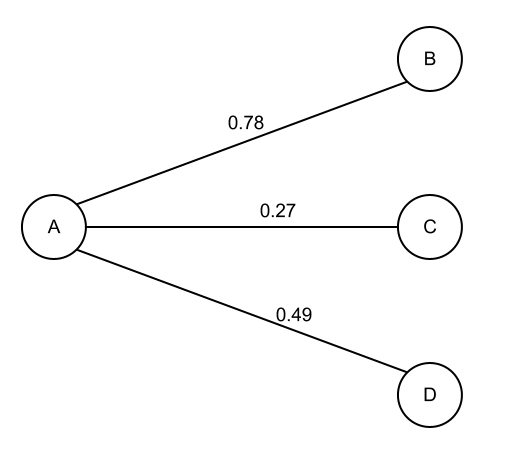
\includegraphics[width=0.5\columnwidth]{images/network}
\caption{A technical network. Contributor A has changed code which contributors B, C and D 
are calling from their own code}
\end{figure}

\subsection{Predicting Success or Failure And Recommendations}
Given a new changeset to a project, we are able to extract all the contributor networks as described
above. After which, we look into the project's past networks to determine if any of the contributor edges have
occurred before and whether or not that edge has a  corresponded to more successful or failed changeset. 

We can now base our prediction of whether a changeset will fail based on this data and we can recommend
high failure rate pairs of contributors communicate during a predicted failed changeset to support the notion
of socio-technical congruence.

\section{Results}
We found a total of X contributor pairs existed over the entire project, of which Y were found to cause
failures inside of the system. We rank failures by the ratio of successful to failed changesets in which 
they were found (Table\ref{tab:ratio}).

\begin{table}[h]
\begin{center}
\begin{tabular}{@{\hspace{.2cm}}ccc@{\hspace{.75cm}}c@{\hspace{.2cm}}}
\hline
Pair & Successful & Failed & Ratio\\
\hline
(Cody, Daisy)	&	0&	12&	1		\\
(Adam, Daisy)	&	1&	14&	0.9697	\\
(Bart, Eve)	&	2&	11&	0.9265      \\
\hline
\end{tabular}
\end{center}
\caption{\label{tab:ratio}}
\end{table}

Using this data, we were able to accurately predict W out of Z failures from a sample size of T given
changesets inside our test project. From these predicted failures we were able to give an average of
H recommendations for contributor communication on average.


\section{Conclusion and Future Work}
It has been shown that technical dependencies are often used as a tool to predict software failures
in large software system\cite{Pinzger:2008:DNP}\cite{Zimmermann:2008:PDU}. 
With this study, we have found evidence that not only can we predict these
failures from technical dependencies themselves, but predict failures based on contributor
dependencies found in changesets over a project's life span. Through the contributor dependencies,
we can also give communication recommendations to contributors that complete the notion of
socio-technical congruence which is also known to increase the probability of changeset success.

Into the future, we will attempt to bring the socio-technical congruence into the foreground of 
our research with the use of actual communication networks on a per commit basis as well. We plan
to investigate the congruence of these social and technical networks and whether or not they 
have an affect on success or failure of builds.



\bibliographystyle{IEEEtran}
\bibliography{paper}


% End of the paper
\end{document}
